\documentclass[10pt]{beamer}
\usetheme[]{AAUsimple}

\setbeamercolor{AAUsimple}{fg=orange!20,bg=orange}
\setbeamercolor{sidebar}{bg=orange!20}
\setbeamercolor{structure}{fg=orange}
\setbeamercolor{frametitle}{fg=white}
\setbeamercolor{normal text}{fg=black,bg=gray!10}

\usepackage[utf8]{inputenc}
\usepackage[french]{babel}
\usepackage[T1]{fontenc}
\usepackage{helvet}


\title{Sécurité Informatique}

\subtitle{Les menaces}

\date{20 Avril 2017}

\author{
  Bouffard-Vercelli Florian\\
  Lee Geertsen
}


\institute[Université des Sciences de Montpellier\\
  Licence Informatique - Deuxième année]
{
  Université des Sciences de Montpellier\\
  Licence Informatique - Deuxième année
}


\pgfdeclareimage[height=1.5cm]{titlepagelogo}{AAUgraphics/Logo_um2.png}
\titlegraphic{
  \pgfuseimage{titlepagelogo}
}

\begin{document}

{\aauwavesbg
\begin{frame}[plain,noframenumbering]
  \titlepage
\end{frame}}


\begin{frame}{Sommaire}{}
\tableofcontents
\end{frame}



\section{Introduction}

\subsection{Sécurité Informatique}

\begin{frame}{Introduction}{Sécurité Informatique}
    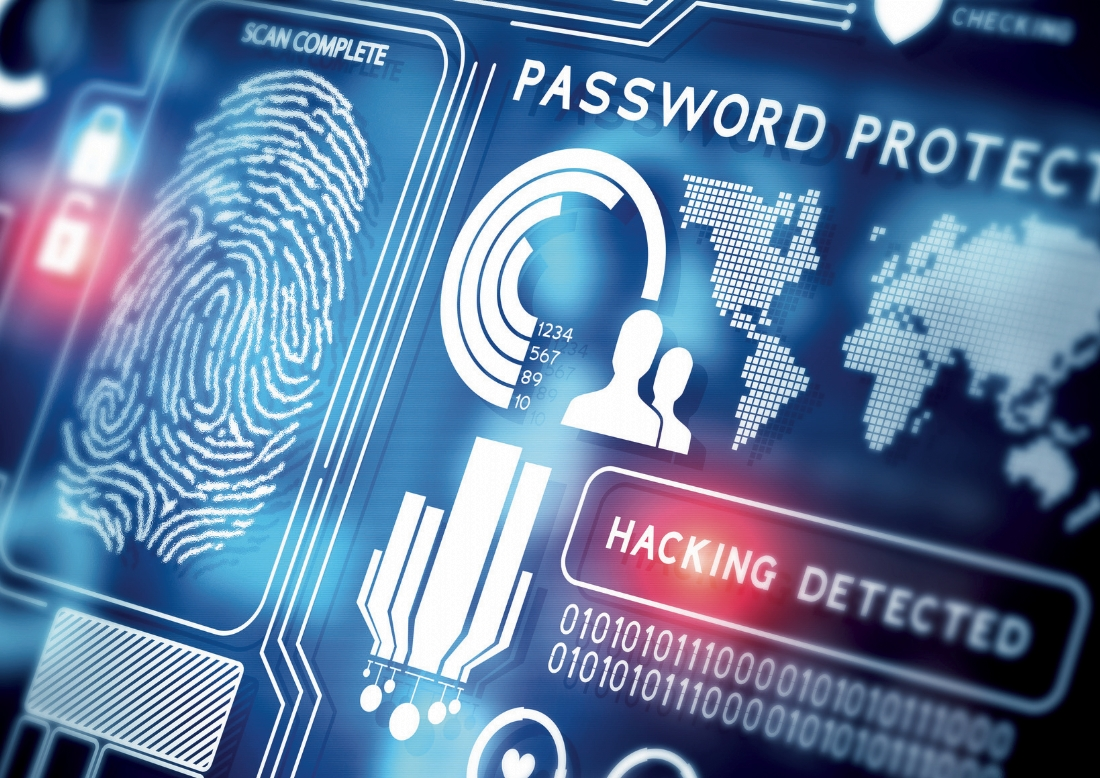
\includegraphics[scale=0.25]{AAUgraphics/Urthawen_Graph/Securite_01.jpg}
\end{frame}
\begin{frame}{Introduction}{Sécurité Informatique}
  \begin{itemize}
    \item<1-> L'intégrité
    \item<2-> La confidentialité
    \item<3-> La disponibilité
    \item<4-> L'authentification
  \end{itemize}
\end{frame}


\subsection{Types d'Authentification forte}

\begin{frame}{Introduction}{Types d'Authentification forte}
    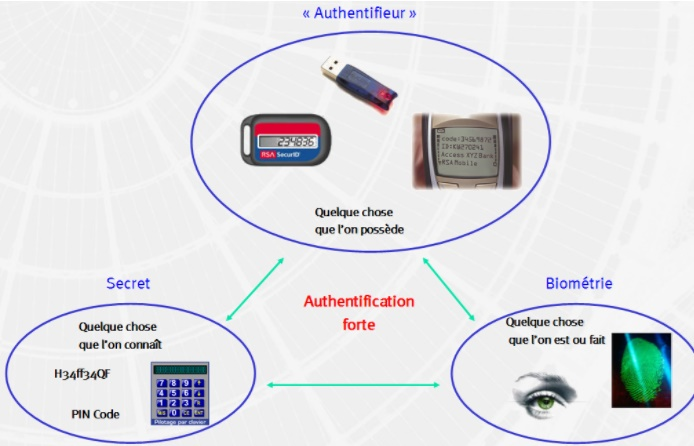
\includegraphics[scale=0.5]{AAUgraphics/Urthawen_Graph/Securite_02.jpg} 
\end{frame}


\section{Les menaces}

\subsection{CoreWar}

\begin{frame}{Les menaces}{CoreWar}
  \begin{block}{Core War}
    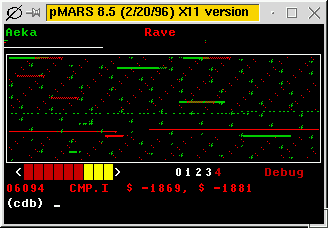
\includegraphics[scale=0.7]{AAUgraphics/Urthawen_Graph/Securite_08.png}  
  \end{block}
\end{frame}

\subsection{Attaque, Fraude, Analyse}

\begin{frame}{Les menaces}{Attaque, Fraude, Analyse}
  \begin{block}{Exploit}
    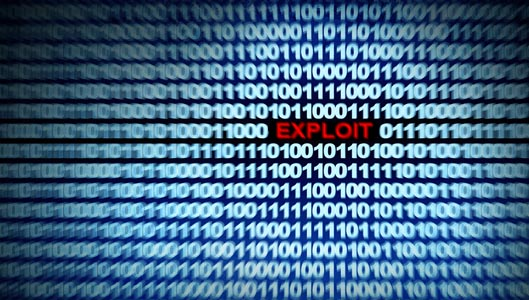
\includegraphics[scale=0.5]{AAUgraphics/Urthawen_Graph/Securite_03.jpg}  
  \end{block}
\end{frame}


\begin{frame}{Les menaces}{Attaque, Fraude, Analyse}
  \begin{block}{Pharming}
    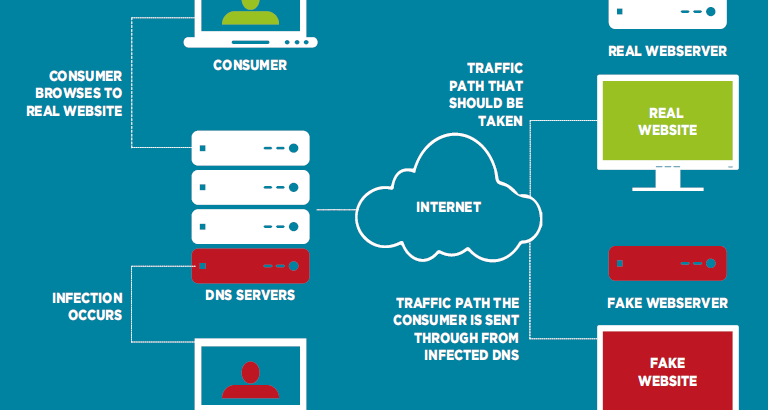
\includegraphics[scale=0.35]{AAUgraphics/Urthawen_Graph/Securite_04.png}    
  \end{block}
\end{frame}

\begin{frame}{Les menaces}{Attaque, Fraude, Analyse}
  \begin{block}{Fork Bomb}
    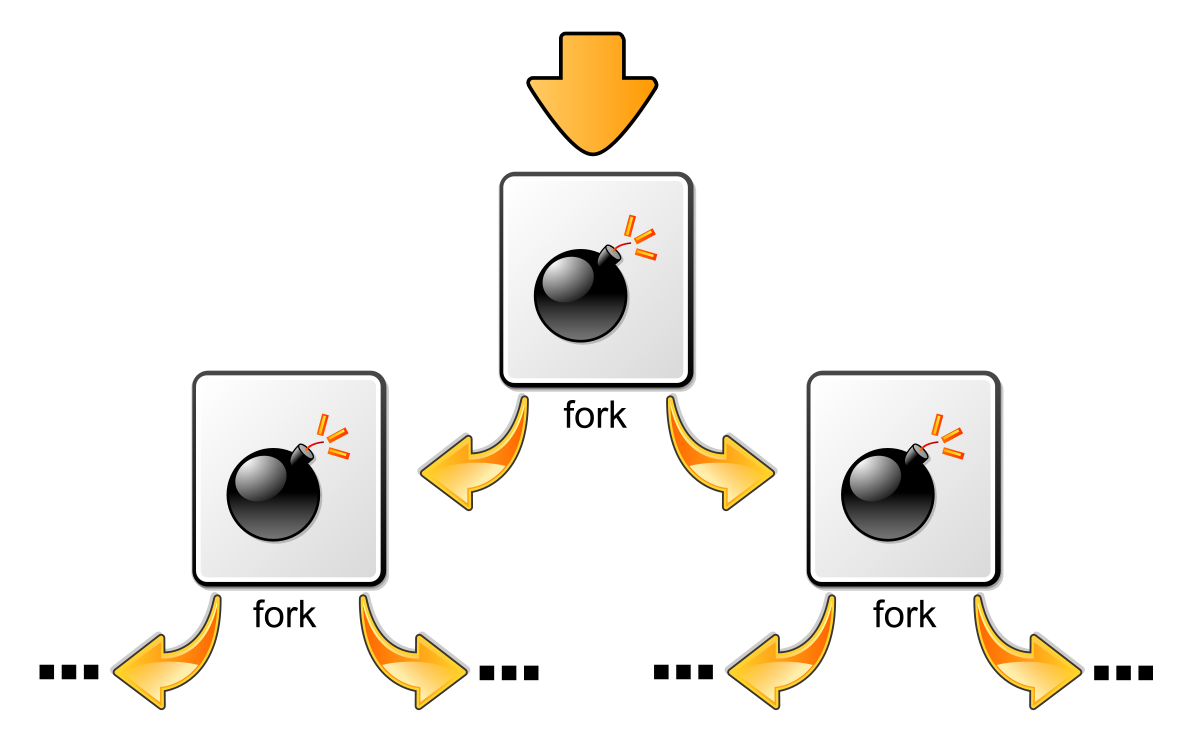
\includegraphics[scale=0.25]{AAUgraphics/Urthawen_Graph/Securite_05.png}    
  \end{block}
\end{frame}

\begin{frame}{Les menaces}{Attaque, Fraude, Analyse}
  \begin{block}{Cross site scripting}
    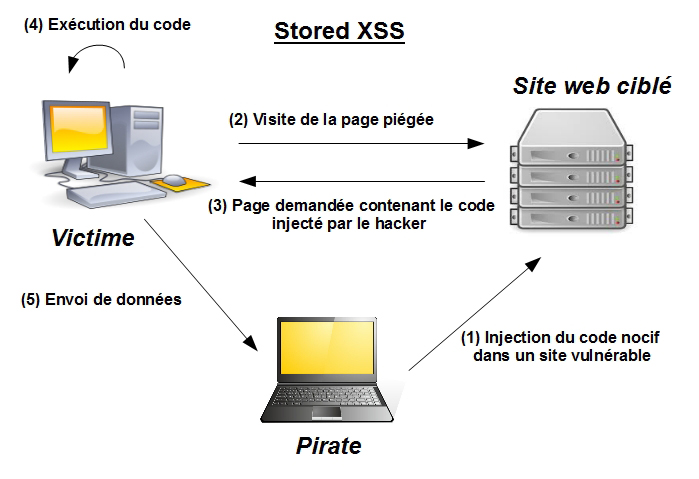
\includegraphics[scale=0.35]{AAUgraphics/Urthawen_Graph/Securite_07.jpg}    
  \end{block}
\end{frame}

\subsection{Malware}

\begin{frame}{{Les menaces}}{Malware}
    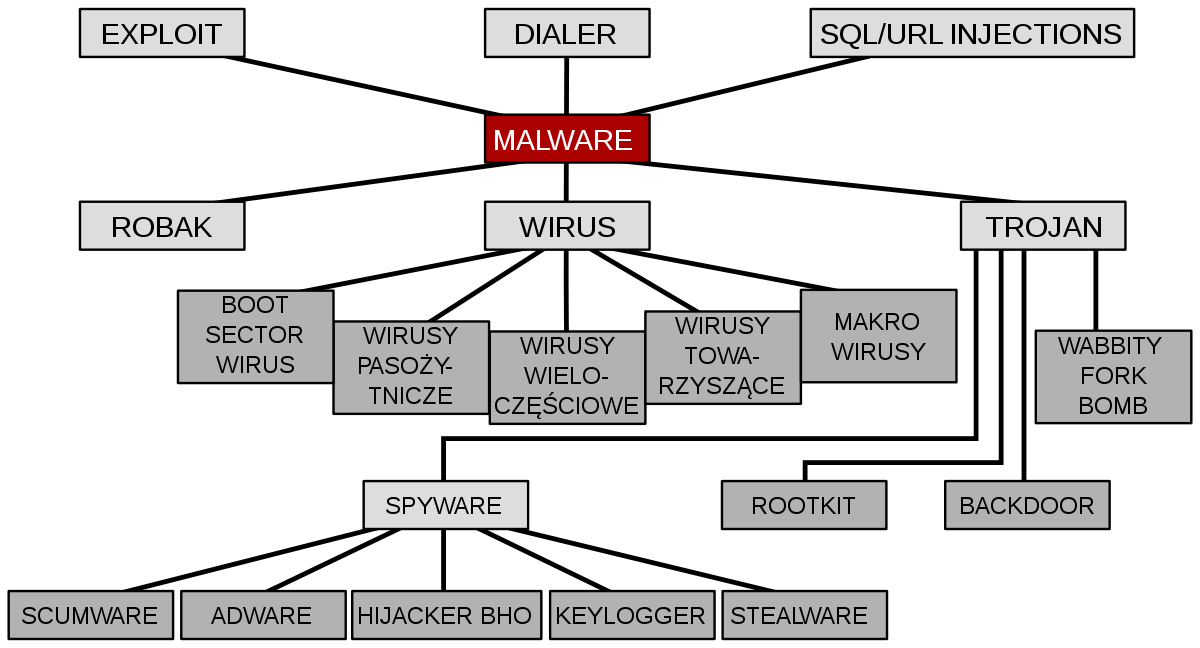
\includegraphics[scale=0.25]{AAUgraphics/Urthawen_Graph/Securite_09.png}  
\end{frame}


\section{Les protections}

\subsection{Les antivirus}

\begin{frame}{Les protections}{Les antivirus}
  \begin{itemize}
    \item<1-> Détecter les virus, vers, troyens, ...
    \item<2-> Existe des tests d'infection sur le web
    \item<3-> Nettoyage
    \item<4-> Antivirus pour tous
  \end{itemize}
\end{frame}

\subsection{Le pare-feu}

\begin{frame}{Les protections}{Le pare-feu}
  \begin{itemize}
    \item<1-> Empêcher l'intrusion
    \item<2-> Empêche le transfert d'un Spyware
  \end{itemize}
\end{frame}

\subsection{La prudence}

\begin{frame}{Les protections}{La prudence}
   \begin{itemize}
    \item<1-> Utiliser des logiciels moins sensibles 
    \item<2-> Eviter les logiciels piratés
    \item<3-> Etre prudent avec les logiciels gratuits
    \item<4-> Eviter les téléchargements sur les réseaux d'échanges de fichiers 
  \end{itemize}
\end{frame}


{\aauwavesbg
\begin{frame}[plain,noframenumbering]
  \finalpage{Merci !}
\end{frame}}

\end{document}
